% !TeX spellcheck = en_GB
% !TeX program = pdflatex
%
% LuxSleek-CV 1.1 LaTeX template
% Author: Andreï V. Kostyrka, University of Luxembourg
%
% 1.1: added tracking and letter-spacing for prettier lower caps, added `~` for language levels
% 1.0: initial release
%
% This template fills the gap in the available variety of templates
% by proposing something that is not a custom class, not using any
% hard-coded settings deeply hidden in style files, and provides
% a handful of custom command definitions that are as transparent as it gets.
% Developed at the University of Luxembourg.
%
% *NOTHING IS HARCODED, and never should be.*
%
% Target audience: applicants in the IT industry, or business in general
%
% The main strength of this template is, it explicitly showcases how
% to break the flow of text to achieve the most flexible right alignment
% of dates for multiple configurations.

\documentclass[11pt, a4paper]{article} 


\usepackage[T1]{fontenc}     % We are using pdfLaTeX,
\usepackage[utf8]{inputenc}  % hence this preparation
\usepackage[british]{babel}  
\usepackage[left = 0mm, right = 0mm, top = 0mm, bottom = 0mm]{geometry}
\usepackage[stretch = 25, shrink = 25, tracking=true, letterspace=30]{microtype}  
\usepackage{graphicx}        % To insert pictures
\usepackage{xcolor}          % To add colour to the document
\usepackage{marvosym}        % Provides icons for the contact details
\usepackage{fontawesome}
\usepackage{setspace}
\usepackage{enumitem}        % To redefine spacing in lists
\setlist{parsep = 0pt, topsep = 0pt, partopsep = 1pt, itemsep = 1pt, leftmargin = 6mm}

\usepackage{FiraSans}        % Change this to use any font, but keep it simple
\renewcommand{\familydefault}{\sfdefault}

\definecolor{cvblue}{HTML}{304263}

%%%%%%% USER COMMAND DEFINITIONS %%%%%%%%%%%%%%%%%%%%%%%%%%%
% These are the real workhorses of this template
\newcommand{\dates}[1]{\hfill\mbox{\textbf{#1}}} % Bold stuff that doesn’t got broken into lines
\newcommand{\is}{\par\vskip.5ex plus .4ex} % Item spacing
\newcommand{\smaller}[1]{{\small$\diamond$\ #1}}
\newcommand{\headleft}[1]{\vspace*{3ex}\textsc{\textbf{#1}}\par%
    \vspace*{-1.5ex}\hrulefill\par\vspace*{0.7ex}}
\newcommand{\headright}[1]{\vspace*{2.5ex}\textsc{\Large\color{cvblue}#1}\par%
     \vspace*{-2ex}{\color{cvblue}\hrulefill}\par}
%%%%%%%%%%%%%%%%%%%%%%%%%%%%%%%%%%%%%%%%%%%%%%%%%%%%%%%%%%%%
\usepackage{fontawesome}
\usepackage[colorlinks = true, urlcolor = magenta, linkcolor = white]{hyperref}

\begin{document}

% Style definitions -- killing the unnecessary space and adding the skips explicitly
\setlength{\topskip}{0pt}
\setlength{\parindent}{0pt}
\setlength{\parskip}{0pt}
\setlength{\fboxsep}{0pt}
\pagestyle{empty}
\raggedbottom

\begin{minipage}[t]{0.33\textwidth} %% Left column -- outer definition
%  Left column -- top dark rectangle
\colorbox{pink}{\begin{minipage}[t][5mm][t]{\textwidth}\null\hfill\null\end{minipage}}

\vspace{-.2ex} % Eliminates the small gap
\colorbox{pink!60}{\color{black}  %% LEFT BOX
\kern0.09\textwidth\relax% Left margin provided explicitly
\begin{minipage}[t][293mm][t]{0.82\textwidth}
\raggedright
\vspace*{2ex}

\textbf{\textsc{Vajihe Mobasheri}} \largesize 

% Centering without extra vertical spacing
\null\hfill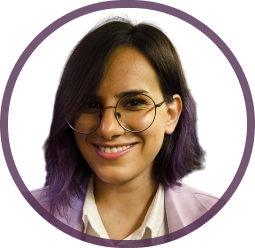
\includegraphics[width=0.95\textwidth]{photo2.png}\hfill\null

\vspace*{1ex} % Extra space after the picture

\headleft{Personal information}
Date of birth: \textbf{13/03/1998} \\[0.5ex]
Citizenship: \textbf{Iran} \\[0.5ex]
Family: \textbf{Single} \\[0.5ex]
Languages: \textbf{English}~(B2), \textbf{Persian}~(native)

\headleft{Research Interest}
\begin{itemize}
\item Artificial Intelligence
\item Design
\item UI/UX
\item Human-AI Collaboration in Design
\end{itemize} 

\headleft{Contact details}
\small % To fit more content
\faEnvelopeO\  \href{mailto:vajihemobasheri76@gmail.com}{vajihemobasheri76@gmail.com} \\[0.1ex]
\faPhone\ +98\,921\,875\,95\, 29 \\[0.5ex]
\faGithub\ \href{https://github.com/VajiheMobasheri}{github.com/VajiheMobasheri} \\[0.1ex]
\faLinkedinSquare\ \href{https://www.linkedin.com/in/vajihe-mobasheri-a2b796231}{linkedin.com/in/VajiheMobasheri} \\[0.1ex]
\faLocationArrow\ Mashhad, Iran
\normalsize



\headleft{Soft Skills}
\begin{itemize}
\item Teamwork
\item Design sense
\item Fast learn
\item Flexibility
\item Good interpersonal skills
\item Active listening 
\end{itemize} 


\headleft{Hobbies}
\begin{itemize}
\item Reading (psychology and Personal Development)
\item Watching movies
\item Gardening 
\item Cooking
\end{itemize} 




\end{minipage}%
\kern0.09\textwidth\relax%%Right margin provided explicitly to stretch the colourbox
}
\end{minipage}% Right column
\hskip2.5em% Left margin for the white area
\begin{minipage}[t]{0.56\textwidth}
\setlength{\parskip}{0.8ex}% Adds spaces between paragraphs; use \\ to add new lines without this space. Shrink this amount to fit more data vertically

% \vspace{2ex}
\headright{Education}
\textbf{\textit{Master of Sciense in Data Sciense}}\\
\faBuilding \ Department of Mathematics\\
\faUniversity \ Ferdowsi University of Mashhad(FUM) \dates{2022.09--pres.} \\
\faLocationArrow \ Mashhad, Iran\\
\smaller \ Thesis title: \textit{Least squares twin support vector machine method with uncertain data} \\
\smaller \ Scientific Experiences: \textit{Supervised learning, Classification, Mathematical optimization} \\
\smaller \ Supervisor: \textit{Dr. Sohrab Effati}\\
\smaller \ Grade: \textit{3.41/4}\\
\smaller \ Thesis defense scheduled for February 18, 2025.
\is
\textbf{\textit{Bachelor of Sciense in Applied Mathematics}}\\
\faBuilding Department of Mathematics\\
\faUniversity Ferdowsi University of Mashhad(FUM) \dates{2016.09--2021.09} \\
\faLocationArrow \ Mashhad, Iran


\headright{Work Experience}
\textbf{\textit{AI Researcher}} \\
\faBuilding \ Faraz Pajohan  \dates{2024.03--pres.} \\
\smaller \ Contributed innovative concepts for AI product UI design to improve usability and aesthetics.\\
\smaller \ Facilitated collaboration with UI/UX designers through structured meetings to align design strategies with product goals.\\
\smaller \ Tailored and optimized the Chainlit interface for AI-driven products to enhance user experience and functionality.\\ 
\smaller \ Crafted detailed and engaging product introduction articles to enhance market awareness and customer understanding.\\
\is 
\textbf{\textit{Business Intelligence Specialist}}\\
\faBuilding \ Faraz Pajohan  \dates{2022.11--2024.3} \\
\smaller \ Conducted data analysis to support strategic decision-making.\\
\smaller \ Designed KPI-based management dashboards using PowerBI to improve operational visibility.\\
\smaller \ Created visually appealing and user-friendly dashboard themes using Figma.\\
\smaller \ Led management meetings to present dashboards, discuss insights, and implement feedback for continuous improvement.


\headright{Skills}
\is
\smaller \ \text{Programming:} \texttt{Python(NumPy, pandas, Vega-Altair, Plotly)}
\is
\smaller \ \text{Web Development:} \texttt{HTML, CSS, JavaScript, React}
\is
\smaller \ \text{AI Frameworks:} \texttt{LangChain/LangGraph(familiar), ChainLit}
\is
\smaller \ \text{Tools:} \texttt{Figma, Git, Power BI, \LaTeX}


% \headright{Projects}
% \textit{Danayar}\\
% \smaller{Developed an AI system called "Danayar" that processes organizational documents and enables a question-answering interface with document referencing at \textit{Faraz Pajohan.}}\dates{2024}\\
% \smaller{Technologies Used: \texttt{LangChain, Chainlit, Retrieval-Augmented Generation(RAG)}}


\headright{Presentation}
\smaller \ {What is Gradient Descent?} \dates{2024}\\
\smaller \  {Attention Is All You Need.} \dates{2023}\\
\smaller \  {What is Elasticsearch?} \dates{2023}\\
\smaller \ {What is Feature Selection?} \dates{2022}\\
\smaller \ {What is PCA and how does it work?} \dates{2022}

\end{minipage}

\newpage
\hskip2.5em% Left margin for the white area
\begin{minipage}[t]{0.90\textwidth}
\setlength{\parskip}{0.8ex}% Adds spaces between paragraphs; use \\ to add new lines without this space. Shrink this amount to fit more data vertically

\vspace{2ex}
\headright{Selected Cources}
\begin{tabular}{l @{\hspace{4cm}} c @{\hspace{1cm}} l @{\hspace{2cm}} c}
\smaller{Big Data} & \textit{3.6/4} & \smaller{Optimization and Neural Networks} & \textit{3.4/4} \\
\smaller{Text Mining} & \textit{3.5/4} & \smaller{Mathematical Foundations of Data Science} & \textit{3.4/4} \\
\smaller{Machine Learning} & \textit{3.4/4} & \smaller{Data Science Algorithms} & \textit{3.4/4} \\
\end{tabular}


\headright{Publications}
\textbf{\textit{Danayar: A Secure and Intelligent Companion for Organizational Managers in Data-Driven Analysis and Decision-Making.}}\dates{2024.09}\\
\smaller{Rasoul Ramezanian;\textcolor{magenta}{Vajihe Mobasheri};  MuhammadReza FatehiNia; Somaye Soltani}\\
\smaller{Type: \textit{Academic-Industrial Research Paper}}\\
\smaller{21\textsuperscript{th} International Conference of the Iranian Society of Cryptology.}


\headright{Certificates}
\textit{Comprehensive Data Science Specialization} \dates{2021--2022}\\
\smaller \ \href{https://ut.ac.ir/en}{Tehran University}\\
\is
\textit{Dashboard design with Microsoft Power BI} \dates{2021}\\
\smaller \ \href{https://mftplus.com/}{Tehran Institute of Technology}


\headright{Other Activities}
\textit{Organized 3 Power BI training workshops.}\\
\faBuilding \ Department of Mathematics\\
\faUniversity \ Ferdowsi University of Mashhad(FUM)  \dates{2021,2022,2024}\\
\smaller \ Scientific Association of Statistics\\
\is
\textit{Delivered Linear Algebra tutorials.}\\
\faYoutubePlay \ YouTube 
\dates{2022}\\
\smaller \ Collaborated with the \href{https://www.linkedin.com/company/data-hub-ir/posts/?feedView=all}{DataHub} team for content development.\\
\is
\textit{Delivered short instructional videos on Power BI.}\\
\faVideoCamera \ \href{https://www.aparat.com/vajihemobasheri}{Aparat (An Iranian video-sharing platform)}
\dates{2021}


\headright{References}
	{\textbf{\href{https://scholar.google.com/citations?hl=en&user=g0onknYAAAAJ}{Prof. Sohrab Effati}}}\\
	\faLocationArrow\ {Ferdowsi University, Mashhad, Iran}{}\\
	\faEnvelopeO\ \href{mailto:s-effati@um.ac.ir}{s-effati@um.ac.ir}\\
	\smaller\ {Prof at Department of Mathematics}{}
    \is
	{\textbf{\href{https://scholar.google.com/citations?user=9kzGRJgAAAAJ&hl=en}{Prof. Omid Soleimani-Frad}}}\\
	\faLocationArrow\ {Ferdowsi University, Mashhad, Iran}{}\\
	\faEnvelopeO\ \href{mailto:soleimani@um.ac.ir}{soleimani@um.ac.ir},\href{mailto:omidsfard@gmail.com}{omidsfard@gmail.com}\\
	\smaller\ {Associated Prof at Department of Mathematics}{}
    \is
	{\textbf{\href{https://scholar.google.com/citations?user=edYFIQEAAAAJ&hl=en}{Prof. Rasoul Ramezanian}}}\\
	\faLocationArrow\ {Lausanne University, Switzerland}{}\\
	\faEnvelopeO\ \href{mailto:rasoul.ramezanian@unil.ch}{rasoul.ramezanian@unil.ch},\href{mailto:rasool.ramezanian@gmail.com}{rasool.ramezanian@gmail.com}\\
	\smaller\ {Senior Researcher at Department of Business and Economics}{}
\end{minipage}
\end{document}
